\title{Initial Management Report}
\author{Nicholas Grasevski \and Daniel Morton \and George El-Boustani \and Christopher Tin-Loi}
\date{\today}

\documentclass{article}
\usepackage{graphicx}
\usepackage{pdfpages}

\begin{document}
\maketitle


\section{Overview}
This document provides a concise analysis of the upcoming Algorithmic Trading System (ATS). It will contain details of our software design and architecture, our development environment, and our initial project plan and milestones, as well as commonly occurring use cases.


\section{Use Cases}
% Develop your initial use cases based on the requirements given (1
% or 2 is enough). Ask the LIC/mentor for clarifications or
% additional information.

\begin{tabular}{|p{1in}|p{3in}|}
\hline
Use Case & Reading a Sirca orders file\\\hline
Description & An orders file is given, and the data is parsed, and translated into trading signals\\
Actors & User\\
Stakeholder & User, Evaluators\\
Preconditions & The file is correctly formatted; i.e. \ contains only buys, sells and trades\\
Postconditions & Order records are generated and are ready to be sent to the trading engine\\
Trigger & A Sirca orders file is given to the parser\\
\hline
\end{tabular}


\section{Design}
\subsection{Architecture Diagram}
% Develop an initial architecture diagram, showing the essential
% components of your system

The architecture diagram below illustrates the preliminary components of the system that we are developing, and the interactions between them. As can be seen, market data will be parsed by the market simulator, which will generate the orders. The market simulator will then forward the orders to the engine, which will maintain the order book and simulate the matching of orders in order to create trades. The same orders will also be forwarded onto the Strategy from the market simulator. The strategy may then generate its own algorithmically generated orders and also send them to the engine. The engine will forward all matched trades to the Strategy Evaluator, which will then analyze and process the trades generating a report that outlines the performance of the given strategy within the market conditions of the provided Sirca data.

\begin{figure}
  \centering
  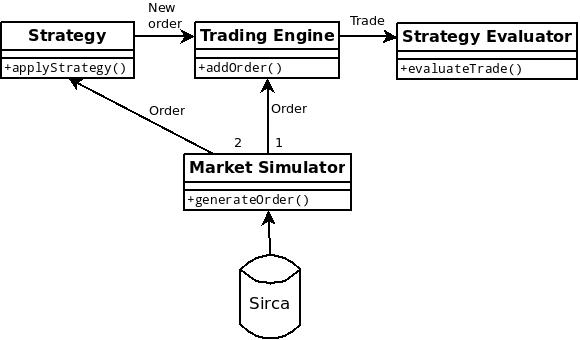
\includegraphics[width=\textwidth]{architecture}
  \caption{Architecture Diagram}
\end{figure}

This architecture is the core logic of our system. For now it can be encapsulated as a batch function which takes in a market data file and displays a strategy evaluation report to the user. Our program is structured such that we have a main library function:
\begin{verbatim}
run_trial(market_data, signal_generator, engine, strategy_evaluator)
\end{verbatim}

which takes in the data file, a signal generator (strategy) plugin, and engine plugin and a strategy evaluator plugin, then runs the simulation and displays the strategy evaluator output (this function also returns the list of trades, so that it can be spooled to a file for example). This library function can then be used by any interface, be it command line, web or GUI\@. A GUI wrapper for example would simply consist of a window to choose the data file and choose and configure the aforementioned plugins, then the user would click ``run" and then once the trial is complete the strategy evaluator plugin would bring up a new window with the results.

\subsection{Interaction and Sequence Diagrams}
% Show interaction or sequence diagrams for each use case defined

\begin{figure}
  \centering
  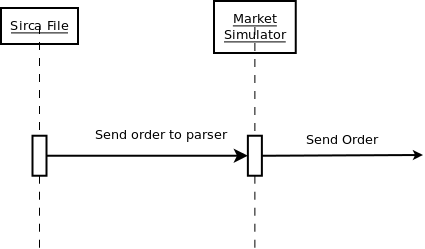
\includegraphics[width=\textwidth]{sequencediagram1}
  \caption{Reading a Sirca orders file}
\end{figure}

\begin{figure}
  \centering
  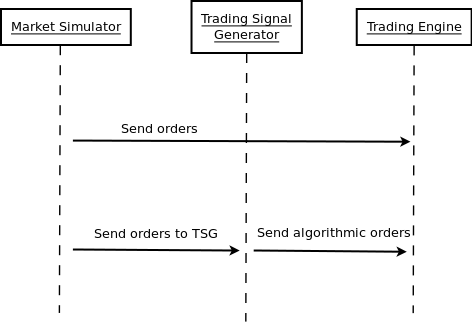
\includegraphics[width=\textwidth]{sequencediagram2}
  \caption{Generating algorithmic orders for one day}
\end{figure}

\begin{figure}
  \centering
  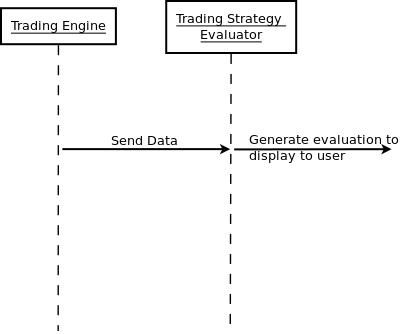
\includegraphics[width=\textwidth]{sequencediagram3}
  \caption{Evaluating algorithmic trades and providing feedback to the user}
\end{figure}



\subsection{Implementation Language and Environment}
% Present and justify implementation language and environment that
% will be used

We have chosen to favor a UNIX environment for our software, but our software is currently and should remain to be cross-compatible across most desktop operating systems such as Windows and Mac OS\@. Our software will be written in Python, for the following reasons:
\begin{description}
  \item[Productivity] Python is a very high level and easy to use language, and its batteries-included nature will aid us in writing quick prototypes.
  \item[Platform Independence] Python's large standard library is mostly platform independent, allowing us to easily port our software to other environments.
  \item[Ubiquity] Python is installed on most UNIX environments by default.
  \item[User Friendliness] By choosing a high level easy to learn scripting language, we can enable users to write their own strategies in Python as plugins, without any further effort of designing a domain-specific language.
  \item[Performance] Python's main resource-intensive libraries are high-performance, and we can leverage this in our scripts. Furthermore if we have performance issues we can always tune the culprit subroutines by rewriting them in C.
  \item[Readability] Python prides itself on its readability, and this will help in coordinating work between team members and reduce the difficulty of understanding each others' code.
  \item[Ease of refactoring] This project is not fully specified, and we are following an Agile process, so refactoring is going to account for a significant portion of the work. Python's avoidance of boilerplate and its general adherence to the DRY principle will help with refactoring.
\end{description}


\section{Project Plan}
% Provide a project plan showing team member responsibilities, work
% arrangements and any information team members will be using to
% coordinate their activities. You should also mention any software
% tools used by the team to assist project management.

Our team is composed of four members. These are our main responsibilities throughout the project:
\begin{description}
  \item[George El Boustani] Tester
  \item[Nicholas Grasevski] Project Manager
  \item[Daniel Morton] Programmer
  \item[Christopher Tin-Loi] Programmer
\end{description}

We will be following an agile development process, with four 2-week sprints:
\begin{description}
  \item[Week 6: a working structure] By this stage, we expect to have the most simple bare bones implementation of the core system working. This excludes GUI and whatnot. Currently we have coded a basic skeleton of our system, and our goal now is to fill in the stubs with the simplest working solutions. I.e. \ our strategy will be random, our engine will only output trades already in the file, and so on.
  \item[Week 8: a simple strategy] Once our structure is in place and working, we hope to iteratively enhance each respective component which requires improvement. This will include improving upon our basic strategy by writing other more sophisticated strategies. Other components of our Algorithmic Trading System will be addressed too. We plan to improve the trading engine incrementally to handle orders in a more realistic manner, and we also plan to improve the strategy evaluator by expanding on the generated evaluation report.
  \item[Week 10: public demo] By this stage we should have our graphical user interface, and it should be streamlined and intuitive for the user.
  \item[Week 12: final demo] By this stage we should have polished all components to an acceptable level.
\end{description}

The project schedule can be found in the appendix. We are currently at the beginning of the first sprint.

We are using various software tools to coordinate our work and to aid in project management:
\begin{description}
  \item[Communication] Currently we communicate primarily through email. Communicating through email gives us a historical record of our interactions and decisions. We also have weekly face to face meetings, phone and sms communication and Internet relay chat communications.
  \item[Version Control] We are using the git VCS to keep track of changes to our code. It allows us to collaborate on our source code tree and record each version. However we haven't limited this to source code and are in fact recording all work including documentation and reports in git, so that we have a record of every change.
  \item[Build System] We also have a build script which compiles all of our source code and documentation and runs all of our tests. We have added this as a pre-commit hook, so that every time somebody commits, all of the documentation is regenerated and all of the tests are run. If any of these steps fail, the commit is rejected. This acts as a sanity check that mitigates the risk of somebody pushing buggy code to the repository. It also ensures that our documentation is kept up to date.
  \item[Source Code Hosting] We have set up a repository on github to enable easier collaboration between our own respective local repositories. We have gone with a centralized model because we are a small team and want to keep things simple. Ideally each of us will regularly pull each others' changes from this repository and push our own changes.
  \item[Issue Tracker] In addition to git hosting, github also provides some basic project management tools. One of these is the issue tracker, which allows one to track feature requests, bugs, milestones and so on. We are currently using this in conjunction with the Gantt chart to track our progress in each sprint, and perhaps in the later stages of development to alert team members of bugs and new requirements. The issue tracker also provides a place to document each task and the ability to comment on an issue provides a record of design decisions made, as well as a concrete interpretation of the requirement.
  \item[Wiki] Github also provides wiki hosting for each project, so we may use this if we find a use for it.
  \item[Code Review] Github enables team members to comment on commits and on tasks, so if a team member finds some dodgy source code, they can either comment on the commit where that dodgy code was introduced or they can comment on the corresponding task in the issue tracker. The culprit is then automatically notified, and they can also respond with a justification for why the code is that way if appropriate.
\end{description}


\appendix
\section{Project Schedule}
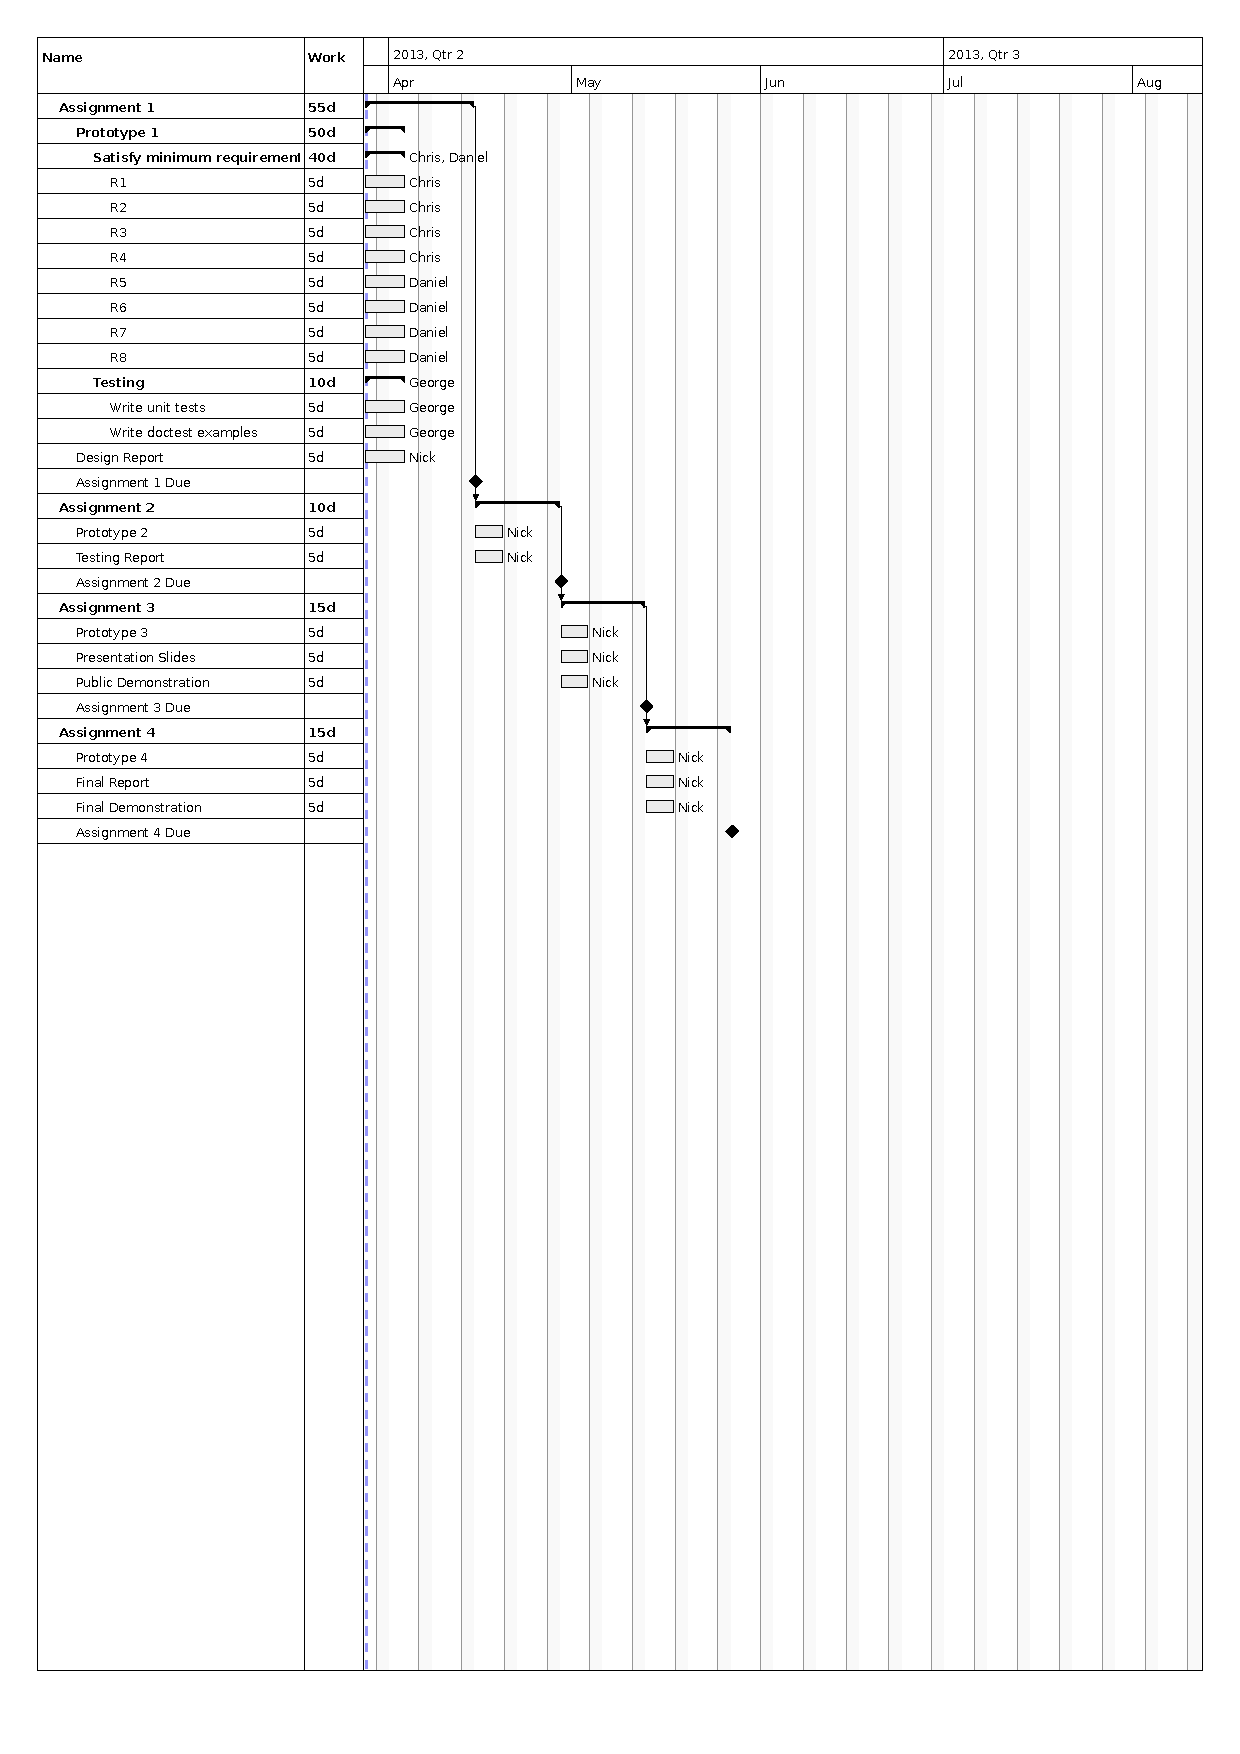
\includepdf[pages={-}]{schedule}

\end{document}
